% !TeX spellcheck = it_IT
\newpage
\section{Elementi basilari}
\subsection{Astrazione}
\begin{wrapfigure}{r}{0.25\textwidth}
	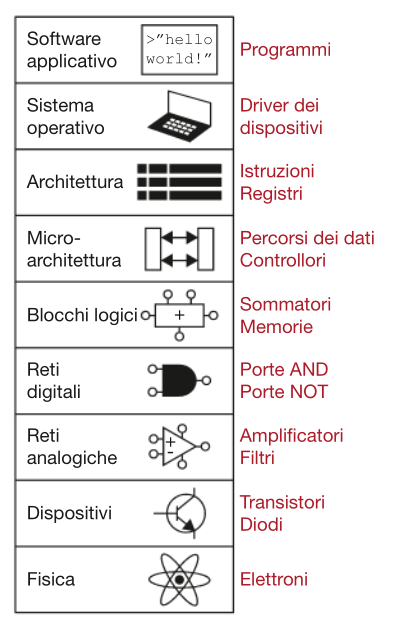
\includegraphics[scale=0.28]{microarchitettura.png}
	\caption{Astrazione di un computer}
\end{wrapfigure}
\begin{definition}[Astrazione]
	La tecnica che consiste nel nascondere dettagli quando questi non sono importanti. Permette di dividere un sistema in più livelli.
\end{definition}

\subsubsection{Tre Y}
Per gestire la complessità i progettisti utilizzano tre principi:
\begin{itemize}
	\item \textbf{Gerarchia}: dividere un sistema in moduli e successivamente dividere questi ultimi finché i pezzi non sono facili da comprendere
	\item \textbf{Modularità}: i moduli hanno funzioni e interfacce ben definite in modo da connettersi semplicemente e senza effetti indesiderati
	\item \textbf{Regolarità}: punta all'uniformità dei moduli, riutilizzando quelli più comuni e riducendo il carico di progettazione
\end{itemize}

\subsubsection{Astrazione digitale}
I sistemi digitali rappresentano le informazioni con variabili \textbf{discrete} che possono avere un numero finito di valori.
\begin{definition}[Quantità di informazione]
	La quantità di informazione $D$ associata a una variabile a valori discreti con $N$ stati distinti è misurata in termini di bit come:
	\begin{equation}
		D = \log_2 N \: bit
	\end{equation}
\end{definition}
Nell'ambito dei calcolatori il numero di valori che può assumere una variabile è due: $0$ o $1$. Queste variabili si basano sulla \textbf{logica Booleana}, dove $0$ rappresenta \textit{FALSO} e $1$ rappresenta \textit{VERO}.

\subsection{Sistemi numerici}
Il sistema da noi utilizzato è quello \textbf{posizionale}, dove ogni possibile valore assume un peso diverso in base alla posizione.
\begin{proposition}[Conversione da base X a base 10]
	Per convertire da una base generica (ad esempio $2$ o $16$) è sufficiente moltiplicare ogni numero per il valore della base elevato alla posizione del numero (partendo da destra).
	\begin{equation*}
		2ED_{16} = 2 \cdot 16^2 + E \cdot 16^1 + D \cdot 16^0 = 749_{10}
	\end{equation*}
\end{proposition}

\begin{proposition}[Conversione da base 10 a base X]
	La conversione da base $10$ ad una base generica consiste nella scomposizione in fattori del numero originale, dalla quale si mantengono i resti:
	\begin{align*}
		333_{10} = \\
		&333 \% 16 = 13 = D_{16} \quad\quad \frac{333}{16} = 20\\
		& 20 \% 16 = 4_{16} \quad\quad \frac{20}{16} = 1 \\
		& 1 \% 16 = 1_{16} \quad\quad \frac{20}{16} = 0 \\
		& = 14D_{16}
	\end{align*}
\end{proposition}

\subsubsection{Unità di misura}
\begin{definition}[Byte]
	Insieme di 8 \textbf{bit}. Rappresenta $2^8=256$ possibilità.
\end{definition}
\begin{definition}[Nibble]
	Un gruppo di 4 \textbf{bit} o mezzo byte. Rappresenta $2^4=16$ possibilità.
\end{definition}
\begin{definition}[Word]
	Sono gruppi di bit utilizzati dai microprocessori la cui grandezza dipende dall'architettura. Ad oggi generalmente sono di $64$ bit.
\end{definition}
\begin{observation}
	All’interno di un gruppo di bit, il bit che si trova nella colonna di peso 1 viene chiamato bit \textbf{meno significativo} (\textit{lsb}, Least Significant Bit) e il bit che si
	trova all’estremità opposta viene chiamato bit \textbf{più significativo} (\textit{msb}, Most Significant Bit). Lo stesso discorso vale per i \textit{byte} (\textit{LSB} e \textit{MSB}).
\end{observation}

\subsubsection{Somma binaria}
La somma binaria avviene esattamente come quella decimale: nel momento in cui due cifre sommate superano il valore massimo $1$, viene scritto $0$ ed effettuato un riporto.
\begin{observation}
	I computer usano sempre un numero fisso di cifre. Di conseguenza se una somma è troppo grande per essere rappresentata, avviene un \textbf{overflow}.
\end{observation}

\subsubsection{Segno}
Per rappresentare il segno di un numero esistono due tecniche:
\begin{itemize}
	\item \textbf{Modulo e segno}: utilizza il \textit{msb} per esprimere il segno e i restanti per il valore del modulo del numero
	\begin{equation*}
		5_{10} = 0101_{2} \quad\quad -5_{10} = 1101_{2}
	\end{equation*}
	Con questo metodo la somma binaria vista in precedente non funziona e abbiamo inoltre due rappresentazioni per lo stesso numero: $-0$ e $0$.
	\item \textbf{Complemento a due}: risolve i problemi dell'altro metodo. I numeri positivi sono rappresentati in maniera classica, con $0$ come \textit{msb}. Quelli negativi si calcolano invertendo bit e aggiungendo $1$.
	\begin{equation*}
		+2_{10} = 0010_2 \quad\quad -2_{10} \to 0010_2 \to 1101_2 \to 1101_2 + 1 = 1110_2
	\end{equation*}
\end{itemize}

\begin{observation}
	Sommare due numeri in complemento a due di segno opposto non causa mai \textbf{overflow}.
\end{observation}

\begin{proposition}[Estensione del segno]
	Quando un numero in complemento a due viene esteso a un numero maggiore di bit, il bit che dà il segno deve essere copiato in tutte le posizioni più significative.
	\begin{equation*}
		-3_{10} = 1011_2 \longrightarrow 1111101_2
	\end{equation*}
\end{proposition}

\subsubsection{Confronto}
Vediamo la \textbf{variabilità} delle rappresentazioni viste fin'ora:
\begin{table}[!h]
	\centering
	\begin{tabular}{|c|c|}
		\hline
		\textbf{Sistema} & \textbf{Range} \\
		\hline
		Senza segno & $[0, 2^N-1]$ \\
		\hline
		Modulo e segno & $[-2^{N-1}, 2^{N-1}-1]$ \\
		\hline
		Complemento a due & $[-2^{N-1}, 2^{N-1}-1]$ \\
		\hline
	\end{tabular}
\end{table}
\newpage
\subsection{Porte logiche}
Le porte logiche (logic gates) sono circuiti digitali che utilizzano uno o più ingressi binari per produrre un’uscita binaria. La relazione tra ingressi e uscite può essere descritta con una \textbf{tabella delle verità} o con una \textbf{espressione booleana}.

\subsubsection{NOT}
\begin{wrapfigure}{r}{0.25\textwidth}
	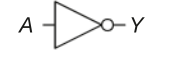
\includegraphics[scale=0.5]{not.png}
\end{wrapfigure}
Ha un ingresso $A$ e un'uscita $Y$: è l'esatto contrario del suo ingresso.
\begin{equation*}
	Y = \bar{A} = \neg A
\end{equation*}

\subsubsection{Buffer}
\begin{wrapfigure}{r}{0.25\textwidth}
	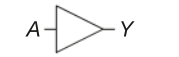
\includegraphics[scale=0.5]{buffer.png}
\end{wrapfigure}
Ha un ingresso $A$ e un'uscita $Y$ e riproduce il valore in ingresso. È utile in particolare dal punto di vista elettrico per erogare grandi quantità di corrente o trasmettere il valore a tante porte logiche diverse.
\begin{equation*}
	Y = A
\end{equation*}

\subsubsection{AND}
\begin{wrapfigure}{r}{0.25\textwidth}
	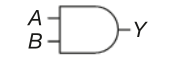
\includegraphics[scale=0.5]{and.png}
\end{wrapfigure}
Ha due ingressi, $A$ e $B$, e restituisce \textit{VERO} solamente se entrambi sono $VERO$, altrimenti $FALSO$.
\begin{equation*}
	Y = AB = A \land B
\end{equation*}
Esiste anche la versione ad $N$ ingressi, dove se tutti sono \textit{VERO} allora il risultato è \textit{VERO}, altrimenti è \textit{FALSO}.

\subsubsection{OR}
\begin{wrapfigure}{r}{0.25\textwidth}
	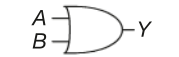
\includegraphics[scale=0.5]{or.png}
\end{wrapfigure}
Ha due ingressi, $A$ e $B$, e restituisce \textit{VERO} se almeno uno dei due è $VERO$, altrimenti $FALSO$.
\begin{equation*}
	Y = A + B = A \lor B
\end{equation*}
Esiste anche la versione ad $N$ ingressi, dove se almeno un ingresso è \textit{VERO} allora il risultato è \textit{VERO}, altrimenti è \textit{FALSO}.

\subsubsection{XOR}
\begin{wrapfigure}{r}{0.25\textwidth}
	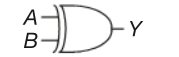
\includegraphics[scale=0.5]{xor.png}
\end{wrapfigure}
Ha due ingressi, $A$ e $B$, e restituisce \textit{VERO} se almeno uno dei due è $VERO$ ma non entrambi, altrimenti $FALSO$.
\begin{equation*}
	Y = A \oplus B
\end{equation*}

\begin{observation}
	Qualunque porta può essere seguita da un pallino per invertire le sue operazioni, ad esempio \textbf{NAND} e \textbf{NOR}.
\end{observation}